% По умолчанию используется шрифт 14 размера. Если нужен 12-й шрифт, уберите опцию [14pt]
\documentclass[14pt
  , russian
  %, xcolor={svgnames}
  ]{matmex-diploma-custom}
\usepackage[table]{xcolor}
\usepackage{graphicx}
\usepackage{tabularx}
\newcolumntype{Y}{>{\centering\arraybackslash}X}
\usepackage{amsmath}
\usepackage{amsthm}
\usepackage{amsfonts}
\usepackage{amssymb}
\usepackage{mathtools}
\usepackage{thmtools}
\usepackage{thm-restate}
\usepackage{tikz}
\usepackage{wrapfig}
% \usepackage[kpsewhich,newfloat]{minted}
% \usemintedstyle{vs}
\usepackage[inline]{enumitem}
\usepackage{subcaption}
\usepackage{caption}
\usepackage[nocompress]{cite}
\usepackage{makecell}
% \setitemize{noitemsep,topsep=0pt,parsep=0pt,partopsep=0pt}
% \setenumerate{noitemsep,topsep=0pt,parsep=0pt,partopsep=0pt}


\graphicspath{ {resources/} }

% 
% % \documentclass 
% %   [ a4paper        % (Predefined, but who knows...)
% %   , draft,         % Show bad things.
% %   , 12pt           % Font size.
% %   , pagesize,      % Writes the paper size at special areas in DVI or
% %                    % PDF file. Recommended for use.
% %   , parskip=half   % Paragraphs: noindent + gap.
% %   , numbers=enddot % Pointed numbers.
% %   , BCOR=5mm       % Binding size correction.
% %   , submission
% %   , copyright
% %   , creativecommons 
% %   ]{eptcs}
% % \providecommand{\event}{ML 2018}  % Name of the event you are submitting to
% % \usepackage{breakurl}             % Not needed if you use pdflatex only.
% 
% \usepackage{underscore}           % Only needed if you use pdflatex.
% 
% \usepackage{booktabs}
% \usepackage{amssymb}
% \usepackage{amsmath}
% \usepackage{mathrsfs}
% \usepackage{mathtools}
% \usepackage{multirow}
% \usepackage{indentfirst}
% \usepackage{verbatim}
% \usepackage{amsmath, amssymb}
% \usepackage{graphicx}
% \usepackage{xcolor}
% \usepackage{url}
% \usepackage{stmaryrd}
% \usepackage{xspace}
% \usepackage{comment}
% \usepackage{wrapfig}
% \usepackage[caption=false]{subfig}
% \usepackage{placeins}
% \usepackage{tabularx}
% \usepackage{ragged2e}
% \usepackage{soul}
\usepackage{csquotes}
% \usepackage{inconsolata}
% 
% \usepackage{polyglossia}   % Babel replacement for XeTeX
%   \setdefaultlanguage[spelling=modern]{russian}
%   \setotherlanguage{english}
% \usepackage{fontspec}    % Provides an automatic and unified interface 
%                          % for loading fonts.
% \usepackage{xunicode}    % Generate Unicode chars from accented glyphs.
% \usepackage{xltxtra}     % "Extras" for LaTeX users of XeTeX.
% \usepackage{xecyr}       % Help with Russian.
% 
% %% Fonts
% \defaultfontfeatures{Mapping=tex-text}
% \setmainfont{CMU Serif}
% \setsansfont{CMU Sans Serif}
% \setmonofont{CMU Typewriter Text}

\usepackage[final]{listings}

\lstdefinelanguage{ocaml}{
keywords={@type, function, fun, let, in, match, with, when, class, type,
nonrec, object, method, of, rec, repeat, until, while, not, do, done, as, val, inherit, and,
new, module, sig, deriving, datatype, struct, if, then, else, open, private, virtual, include, success, failure,
lazy, assert, true, false, end},
sensitive=true,
commentstyle=\small\itshape\ttfamily,
keywordstyle=\ttfamily\bfseries, %\underbar,
identifierstyle=\ttfamily,
basewidth={0.5em,0.5em},
columns=fixed,
fontadjust=true,
literate={->}{{$\to$}}3 {===}{{$\equiv$}}1 {=/=}{{$\not\equiv$}}1 {|>}{{$\triangleright$}}3 {\\/}{{$\vee$}}2 {/\\}{{$\wedge$}}2 {>=}{{$\ge$}}1 {<=}{{$\le$}} 1,
morecomment=[s]{(*}{*)}
}

\lstset{
mathescape=true,
%basicstyle=\small,
identifierstyle=\ttfamily,
keywordstyle=\bfseries,
commentstyle=\scriptsize\rmfamily,
basewidth={0.5em,0.5em},
fontadjust=true,
language=ocaml
}
 
\newcommand{\cd}[1]{\texttt{#1}}
\newcommand{\inbr}[1]{\left<#1\right>}


\newcolumntype{L}[1]{>{\raggedright\let\newline\\\arraybackslash\hspace{0pt}}m{#1}}
\newcolumntype{C}[1]{>{\centering\let\newline\\\arraybackslash\hspace{0pt}}m{#1}}
\newcolumntype{R}[1]{>{\raggedleft\let\newline\\\arraybackslash\hspace{0pt}}m{#1}}



\usepackage{soul}
\usepackage[normalem]{ulem}
%\sout{Hello World}

% перевод заголовков в листингах
\renewcommand\lstlistingname{Листинг}
\renewcommand\lstlistlistingname{Листинги}

\usepackage{afterpage}
\usepackage{pdflscape}

\begin{document}
%% Если что-то забыли, при компиляции будут ошибки Undefined control sequence \my@title@<что забыли>@ru
%% Если англоязычная титульная страница не нужна, то ее можно просто удалить.
\filltitle{ru}{
    %% Актуально только для курсовых/практик. ВКР защищаются не на кафедре а в ГЭК по направлению, 
    %%   и к моменту защиты вы будете уже не в группе.
    chair              = {Кафедра системного программирования},
    group              = {19Б.10-мм},
    %
    %% Макрос filltitle ненавидит пустые строки, поэтому обязателен хотя бы символ комментария на строке
    %% Актуально всем.
    title              = {Разработка алгоритма для задачи достижимости с регулярными ограничениями},
    % 
    %% Здесь указывается тип работы. Возможные значения:
    %%   coursework - отчёт по курсовой работе;
    %%   practice - отчёт по учебной практике;
    %%   prediploma - отчёт по преддипломной практике;
    %%   master - ВКР магистра;
    %%   bachelor - ВКР бакалавра.
    type               = {practice},
    %
    %% Здесь указывается вид работы. От вида работы зависят критерии оценивания.
    %%   solution - <<Решение>>. Обучающемуся поручили найти способ решения проблемы в области разработки программного обеспечения или теоретической информатики с учётом набора ограничений.
    %%   experiment - <<Эксперимент>>. Обучающемуся поручили изучить возможности, достоинства и недостатки новой технологии, платформы, языка и т. д. на примере какой-то задачи.
    %%   production - <<Производственное задание>>. Автору поручили реализовать потенциально полезное программное обеспечение.
    %%   comparison - <<Сравнение>>. Обучающемуся поручили сравнить несколько существующих продуктов и/или подходов.
    %%   theoretical - <<Теоретическое исследование>>. Автору поручили доказать какое-то утверждение, исследовать свойства алгоритма и т.п., при этом не требуя написания кода.
    kind               = {solution},
    %
    author             = {Порсев Денис Витальевич},
    % 
    %% Актуально только для ВКР. Указывается код и название направления подготовки. Типичные примеры:
    %%   02.03.03 <<Математическое обеспечение и администрирование информационных систем>>
    %%   02.04.03 <<Математическое обеспечение и администрирование информационных систем>>
    %%   09.03.04 <<Программная инженерия>>
    %%   09.04.04 <<Программная инженерия>>
    %% Те, что с 03 в середине --- бакалавриат, с 04 --- магистратура.
    specialty          = {02.03.03 <<Математическое обеспечение и администрирование информационных систем>>},
    % 
    %% Актуально только для ВКР. Указывается шифр и название образовательной программы. Типичные примеры:
    %%   СВ.5006.2017 <<Математическое обеспечение и администрирование информационных систем>>
    %%   СВ.5162.2020 <<Технологии программирования>>
    %%   СВ.5080.2017 <<Программная инженерия>>
    %%   ВМ.5665.2019 <<Математическое обеспечение и администрирование информационных систем>>
    %%   ВМ.5666.2019 <<Программная инженерия>>
    %% Шифр и название программы можно посмотреть в учебном плане, по которому вы учитесь. 
    %% СВ.* --- бакалавриат, ВМ.* --- магистратура. В конце --- год поступления (не обязательно ваш, если вы были в академе/вылетали).
    programme          = {СВ.5006.2017 <<Математическое обеспечение и администрирование информационных систем>>},
    % 
    %% Актуально только для ВКР, только для матобеса и только 2017-2018 годов поступления. Указывается профиль подготовки, на котором вы учитесь.
    %% Названия профилей можно найти в учебном плане в списке дисциплин по выбору. На каком именно вы, вам должны были сказать после второго курса (можно уточнить в студотделе).
    %% Вот возможные вариканты:
    %%   Математические основы информатики
    %%   Информационные системы и базы данных
    %%   Параллельное программирование
    %%   Системное программирование
    %%   Технология программирования
    %%   Администрирование информационных систем
    %%   Реинжиниринг программного обеспечения
    % profile            = {Системное программирование},
    % 
    %% Актуально всем.
    %supervisorPosition = {проф. каф. СП, д.ф.-м.н., проф.}, % Терехов А.Н.
    supervisorPosition = {доцент кафедры информатики, к.ф.-м.н.,}, % Григорьев С.В.
    supervisor         = {Григорьев С.В.}
    % 

    % consultantPosition = {должность ООО <<Место работы>> степень},
    % consultant         = {К.К. Консультант}
}

\maketitle
\setcounter{tocdepth}{3}
\tableofcontents

% \begin{abstract}
%   В курсаче не нужен
% \end{abstract}

\section{Introduction}

Scalable high-performance graph analysis is an actual challenge.
There is a big number of ways to attack this challenge~\cite{Coimbra2021} and the first promising idea is to utilize general-purpose graphic processing units (GPGPU-s).
Such existing solutions, as CuSha~\cite{10.1145/2600212.2600227} and Gunrock~\cite{7967137} show that utilization of GPUs can improve the performance of graph analysis, moreover it is shown that solutions may be scaled to multi-GPU systems.
But low flexibility and high complexity of API are problems of these solutions.

The second promising thing which provides a user-friendly API for high-performance graph analysis algorithms creation is a GraphBLAS API~\cite{7761646} which provides linear algebra based building blocks to create graph analysis algorithms.
The idea of GraphBLAS is based on is a well-known fact that linear algebra operations can be efficiently implemented on parallel hardware.
Along with this, a graph can be natively represented using matrices: adjacency matrix, incidence matrix, etc.
While reference CPU-based implementation of GraphBLAS, SuiteSparse:GraphBLAS~\cite{10.1145/3322125}, demonstrates good performance in real-world tasks, GPU-based implementation is challenging.

One of the challenges in this way is that real data are often sparse, thus underlying matrices and vectors are also sparse, and, as a result, classical dense data structures and respective algorithms are inefficient. 
So, it is necessary to use advanced data structures and procedures to implement sparse linear algebra, but the efficient implementation of them on GPU is hard due to the irregularity of workload and data access patterns.
Though such well-known libraries as cuSparse show that sparse linear algebra operations can be efficiently implemented for GPGPU-s, it is not so trivial to implement GraphBLAS on GPGPU. 
First of all, it requires \textit{generic} sparse linear algebra, thus it is impossible just to reuse existing libraries which are almost all specified for operations over floats.
The second problem is specific optimizations, such as maskings fusion, which can not be natively implemented on top of existing kernels.
Nevertheless, there is a number of implementations of GraphBLAS on GPGPU, such as GraphBLAST:~\cite{yang2019graphblast}, GBTL~\cite{7529957}, which show that GPGPUs utilization can improve the performance of GraphBLAS-based graph analysis solutions.
But these solutions are not portable because they are based on Nvidia Cuda stack.
Moreover, the scalability problem is not solved: all these solutions support only single-GPU, not multi-GPU computations.

To provide portable GPU implementation of GraphBLAS API we developed a \textit{SPLA} library (sources are published on GitHub: \url{https://github.com/JetBrains-Research/spla}).
This library utilizes OpenCL for GPGPU computing to be portable across devices of different vendors.
Moreover, it is initially designed to utilize multiple GPGPUs to be scalable.
To sum up, the contribution of this work is the following.
\begin{itemize}
    \item Design of portable GPU GraphBLAS implementation proposed. The design involves the utilization of multipole GPUS. Additionally, the proposed design is aimed to simplify library tuning and wrappers for different high-level platforms and languages creation. 
    \item Subset of GraphBLAS API, including such operations as masking, matrix-matrix multiplication, matrix-matrix e-wise addition, is implemented. The current implementation is limited by COO and CSR matrix representation format and uses basic algorithms for some operations, but work in progress and more data formats will be supported and advanced algorithms will be implemented in the future.
    \item Preliminary evaluation on such algorithms as breadth-first search (BFS) and triangles counting (TC), and real-world graphs shows portability across different vendors and promising performance: for some problems Spla is comparable with GraphBLAST. Surprisingly, for some problems, the proposed solution on embedded Intel graphic card shows better performance than SuiteSparse:GraphBLAS on the same CPU. At the same time, the evaluation shows that further optimization is required.
\end{itemize} 
\section{Цель и задачи}

Целью данной работы является реализация алгоритма поиска путей в графовых базах данных через тензорное произведение на GPGPU. Для ее выполнения были поставлены следующие задачи.

\begin{itemize}
    \item Разработка архитектуры библиотеки примитивов разреженной линейной булевой алгебры для вычислений на GPGPU.
    \item Реализация библиотеки в соответствии с разработанной архитектурой.
    \item Реализация алгоритма поиска путей с КС ограничениями через тензорное произведение с использованием разработанной библиотеки.
    \item Экспериментальное исследование библиотеки и реализации алгоритма.
\end{itemize}
\section{Обзор предметной области}

Для разработки библиотеки и реализации нового алгоритма необходимо сперва рассмотреть базовую теорию запросов к графам с КС ограничениями, а также ознакомиться с существующими подходами к реализации.
Для этого предлагается рассмотреть алгоритмы выполнения данных запросов, с акцентом на перспективное направление алгоритмов, которые полагаются на операции разреженной линейной алгебры. Необходимо рассмотреть алгоритм поиска путей на основе тензорного произведения, а также существующие инструменты для работы с примитивами разреженной линейной алгебры на GPU. Это поможет обосновать необходимость разработки нового подобного инструмента.

\subsection{Терминология}

% В этой секции изложены основные определения и факты из теории графов и формальных языков, необходимые для понимания предметной области. 
    
\textit{Ориентированный граф с метками на ребрах} $\mathcal{G} = \langle V, E, L \rangle$ это тройка объектов, где $V$ конечное непустое множество вершин графа, $E \subseteq V \times L \times V$ конечное множество ребер графа, $L$ конечное множество меток графа. Здесь и далее будем считать, что вершины графа индексируются целыми числами, т.е. $V = \{0~,...,~|V| - 1\}$.

Граф $\mathcal{G} = \langle V, E, L \rangle$ можно представить в виде матрицы смежности $M$ размером $|V| \times |V|$, где $M[i,j] = \{l~|~(i,l,j) \in E\}$. Используя булеву матричную декомпозицию, можно представить матрицу смежности в виде набора матриц $\mathcal{M} = \{ M^l ~|~ l \in L, M^l[i,j] = 1 \iff l \in M[i,j]\}$.

Путь $\pi$ в графе $\mathcal{G} = \langle V, E, L \rangle$ это последовательность ребер $e_0,e_1,e_{n-1}$, где $e_i = (v_i, l_i, u_i) \in E$ и для любых $e_i, e_{i+1}: u_i = v_{i+1}$. Путь между вершинами $v$ и $u$ будем обозначать как $v \pi u$. Слово, которое формирует путь $\pi = (v_0, l_0, v_1), ... ,(v_{n-1}, l_{n-1}, v_n)$ будем обозначать как $\omega (\pi) = l_0 ... l_{n-1}$, что является конкатенацией меток вдоль этого пути $\pi$.

\textit{Контекстно-свободная (КС) грамматика} $G = \langle \Sigma, N, P, S \rangle$ это четверка объектов, где $\Sigma$ конечное множестве терминалов или терминальный алфавит, $N$ конечное множество нетерминалов, $P$ конечное множество правил вывода вида $A \rightarrow \gamma, \gamma \in (N \cup \Sigma)^*$, $S \in N$ стартовый нетерминал. Вывод слова $w$ в грамматике из нетерминала $S$ применением одного или нескольких правил вывода обозначается как $S \rightarrow^*_G w$.

Язык $\mathcal{L}$ над конечным алфавитом символов $\Sigma$ --- множество слов, составленных из символов этого алфавита, т.е. $\mathcal{L} \subseteq \{w~|~w \in \Sigma ^*\}$. Язык, задаваемый грамматикой $G$, обозначим как $\mathcal{L}(G) = \{w~|~S \rightarrow^*_G w\}$.

\textit{Произведение Кронекера} матриц $A$ и $B$ с размером $m \times n$ и $p \times q$ соответственно это блочная матрица размера $mp \times nq$, где блок с индексом $(i,j)$ вычисляется как $a_{ij} * B$.

% Keep this thing commented
% \begin{figure}[h]
%     \centering
%     \begin{subfigure}[b]{0.50\textwidth}
%         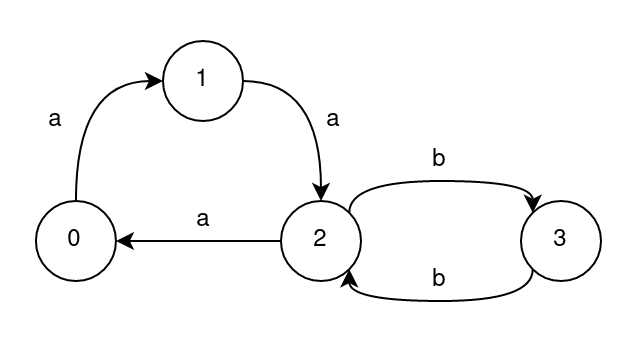
\includegraphics[width=\textwidth]{images/example_graph.png}
%         \caption{Ориентированный граф с меткам}
%     \end{subfigure}
%     \hfill
%     \begin{subfigure}[b]{0.20\textwidth}
%         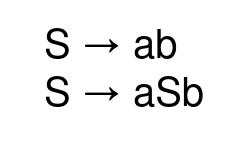
\includegraphics[width=\textwidth]{images/exmample_grammar.png}
%         \caption{Грамматика}
%     \end{subfigure}
%     \caption{Пример графа и грамматики}
% \end{figure}

\subsection{Поиск путей с ограничениями}

При вычислении запроса на поиск путей в графе $\mathcal{G} = \langle V, E, L \rangle$ в качестве ограничения выступает некоторый язык $\mathcal{L}$, которому должны удовлетворять результирующие пути.

Поиск путей в графе с семантикой \textbf{достижимости} --- это поиск всех таких пар вершин $(v,u)$, что между ними существует путь $v \pi u$ такой, что $\omega (\pi) \in \mathcal{L}$. Результат запроса обозначается как $R = \{ (v,u)~|~\exists v \pi u : \omega (\pi) \in \mathcal{L} \}$.

Поиск путей в графе с семантикой \textbf{всех путей} --- это поиск всех таких путей $v \pi u$,   что $\omega (\pi) \in \mathcal{L}$. Результат запроса обозначается как $\Pi = \{ v \pi u~|~v \pi u : \omega (\pi) \in \mathcal{L} \}$.
Необходимо отметить, что множество $\Pi$ может быть бесконечным, поэтому в качестве результата запроса предполагается не всё множество в явном виде, а некоторый \textit{итератор}, который позволит последовательно извлекать все пути.

Семантика \textbf{одного пути} является ослабленной формулировкой семантики всех путей, так как для получения результата достаточно найти всего один путь вида $v \pi u : \omega (\pi) \in \mathcal{L}$ для каждой пары $(v, u) \in R$.

Поскольку язык $\mathcal{L}$ может быть бесконечным, при составлении запросов используют не множество $\mathcal{L}$ в явном виде, а некоторое правило формирования слов этого языка. В качестве таких правил и выступают регулярные выражения или КС грамматики. При именовании запросов отталкиваются от типа правил, поэтому запросы именуются как регулярные или КС соответственно.

\subsection{Существующие решения}

Впервые проблема выполнения запросов с контекстно-свободными ограничениями была сформулирована в 1990 году в работе Михалиса Яннакакиса~\cite{inproceedings:yannakakis_cfpq_problem}. С того времени были представлены многие работы, в которых так или иначе предлагалось решение данной проблемы. 

Однако недавно  Йохем Куиджперс и др.~\cite{article:kuijpers_cfpq_exp_compare} на основе сравнения нескольких алгоритмов~\cite{article:hellings_cfpq,inproceedings:matrix_cfpq,inbook:santos_cfpq_lr_analysis} для выполнения запросов с контекстно-свободными ограничениями заключили, что существующие алгоритмы неприменимы для практики из-за проблем с производительностью.
Стоит отметить, что алгоритмы, используемые в статье, были реализованы на языке программирования \textit{Java} и исполнялись в среде \textit{JVM} в однопоточном режиме, что могло существенно повлиять на производительность представленных алгоритмов и, соответственно, выводы авторов.

Это подтверждают результаты работы Арсения Терехова и др.~\cite{inproceedings:cfqp_matrix_with_single_source}, в которой с использованием программных и аппаратных средств Nvidia Cuda был реализован алгоритм Рустама Азимова~\cite{inproceedings:matrix_cfpq}. В данном алгоритме задача поиска путей с КС ограничениями была сведена к операциям линейной алгебры, что позволило использовать высокопроизводительные библиотеки для выполнения данных операций на GPGPU. 
Данное исследование показало, что эффективная реализация алгоритма на GPU может сделать его применимым для анализа реальных данных.


Алгоритм Рустама Азимова~\cite{inproceedings:cfqp_matrix_with_single_source} способен выполнять запросы только в семантике одного пути. Поскольку в качестве формализма для представления грамматики КС запроса используется \textit{ослабленная нормальная форма Хомского (ОНФХ)}~\cite{book:automata_theory}, увеличение числа правил в исходной грамматике запроса может приводить к существенному разрастанию ОНФХ, что негативно влияет на время работы алгоритма.

\subsection{Поиск путей с КС ограничениями через тензорное произведение}

Представленный в работе Егора Орачева и др.~\cite{inbook:kronecker_cfpq_adbis} алгоритм для выполнения КС запросов использует операции линейной булевой алгебры: произведение Кронекера (частный случай тензорного произведения), матричное умножение и сложение. Данный алгоритм позволяет выполнять запросы в семантике достижимости и всех путей, а также он подходит для реализации на многоядерных системах, что делает его потенциально применимым для анализа реальных данных. Кроме этого, данный алгоритм использует в качестве формализма для представления запроса \textit{рекурсивный автомат} (РА)~\cite{article:recursive_state_machines}, что потенциально может решить проблему разрастания исходной грамматики запроса. 

Идея алгоритма состоит в \textit{пересечении} РА и графа с использованием некоторой модификации классического алгоритма пересечения конечных автоматов~\cite{book:automata_theory}. Пересечение выполняется с использованием произведения Кронекера, а множество рекурсивных вызовов учитывается с помощью транзитивного замыкания, что также выражается с использованием матричных операций умножения и поэлементного сложения. Данный процесс итеративный, и он выполняется до тех пор, пока в результирующий граф добавляются новые ребра.

% Далее предлагается рассмотреть описание данного алгоритма и используемую им технику сведения вычислений к операциям линейной алгебры.

% \subsubsection*{Рекурсивный автомат}

% Для представления входной грамматики КС запроса алгоритм~\cite{inbook:kronecker_cfpq_adbis} использует \textit{рекурсивный автомат}. Данный формализм является своего рода обобщением \textit{недетерминированного конечного автомата} на случай КС языков. Для понимания того, как он устроен, обратимся к теории формальных языков.

% \textit{Недетерминированный конечный автомат} (НКА) $F = \langle \Sigma, Q, Q_s, Q_f, \delta \rangle$ это пятерка объектов, где:

% \begin{itemize}
%     \item $\Sigma$ конечное множество входных символов или алфавит
%     \item $Q$ конечное множество состояний
%     \item $Q_s \subseteq Q$ множество стартовых состояний
%     \item $Q_f \subseteq Q$ множество конечных состояний
%     \item $\delta : \Sigma \times Q \rightarrow 2^Q$ функция переходов автомата
% \end{itemize}

% Язык, допускаемый автоматом $F$ будем обозначать как $L(F)$. Любое регулярное выражение может быть преобразовано в соответствующий НКА~\cite{book:automata_theory}. 

% \textit{Рекурсивный автомат} (РА) $R = \langle M, m, \{C_i\}_{i \in M} \rangle$ это тройка объектов, где: 

% \begin{itemize}
%     \item $M$ конечное множество меток компонентных НКА, называемых далее \textit{модули}
%     \item $m$ метка стартового модуля
%     \item $\{C_i\}$ множество модулей, где модуль $C_i = \langle \Sigma \cup M, Q_i, S_i, F_i, \delta _i \rangle$ состоит из:
%     {
%     \begin{itemize}
%         \item $\Sigma \cup M$ множество символов модуля, $\Sigma \cap M = \emptyset$
%         \item $Q_i$ конечное множество состояний модуля, $Q_i \cap Q_j = \emptyset, \forall i \neq j$
%         \item $S_i \subseteq Q_i$ множество стартовых состояний модуля
%         \item $F_i \subseteq Q_i$ множество конечных состояний модуля 
%         \item $\delta_i : (\Sigma \cup M) \times Q_i \rightarrow 2^{Q_i}$ функция переходов
%     \end{itemize}
%     }
% \end{itemize}

% Рекурсивный автомат ведет себя как набор НКА или модулей~\cite{article:recursive_state_machines}. Эти модули очень сходны с НКА при обработке входных последовательностей символов, однако они способны обрабатывать дополнительные \textit{рекурсивные вызовы} за счет неявного \textit{стека вызовов}, который присутствует во время работы РА. С точки зрения прикладного программиста это похоже на рекурсивные вызовы одних функций из других с той разницей, что вместо функций здесь выступают модули РА.

% Рекурсивные автоматы по своей вычислительной мощности эквивалентны магазинным автоматам~\cite{article:recursive_state_machines}. А поскольку подобный магазинный автомат способен распознавать КС грамматику~\cite{book:automata_theory}, рекурсивные автоматы эквивалентны КС грамматикам. Это позволяет корректно использовать РА для представления входной КС грамматики запроса.

% \subsubsection*{Пересечение рекурсивного автомата и графа}

% Классический алгоритм~\cite{book:automata_theory} \textit{пересечения} двух НКА $F^1$ и $F^2$ позволяет построить новый НКА $F$ с таким свойством, что он допускает пересечение исходных регулярных языков, т.е. $L(F) = L(F^1) \cap L(F^2)$. Формально, для $F^1 = \langle \Sigma, Q^1, Q^1_S, Q^1_F, \delta^1 \rangle$ и $F^2 = \langle \Sigma, Q^2, Q^2_S, Q^2_F, \delta^2 \rangle$ строится новый НКА $F = \langle \Sigma, Q, Q_S, Q_F, \delta \rangle$, где:

% \begin{itemize}
%     \item $Q = Q^1 \times Q^2$
%     \item $Q_S = Q^1_S \times Q^2_S$
%     \item $Q_F = Q^1_F \times Q^2_F$
%     \item $\delta: \Sigma \times Q \rightarrow Q$ и $\delta(s, \langle q_1, q_2 \rangle) = \langle q'_1, q'_2 \rangle$, если $\delta^1 (s, q_1)=q'_1$ и $\delta^2 (s, q_2)=q'_2$ 
% \end{itemize}

% Интерпретируя ориентированный граф с метками как некоторый конечный автомат, в котором все вершины графа являются одновременно начальными и конечными состояниями автомата, а ребра графа --- переходами между состояниями автомата, возможно пересечь этот граф и некоторый НКА, используя алгоритм пересечения, описанный выше. Однако, если представить граф и функцию переходов КА, тоже интерпретируемую как граф, в виде матриц смежности, можно использовать \textit{произведение Кронекера} для построения функции переходов автомата пересечения.

% \textit{Произведение Кронекера} для двух матриц $A$ и $B$ размера $m_1 \times n_1$ и $m_2 \times n_2$ с поэлементной операцией умножения $\cdot$ дает матрицу $M = A \otimes B$ размером $m_1 * m_2 \times n_1 * n_2$, где $M[u * m_2 + v, p * n_2 + q] = A[u, p] \cdot B[v, q]$. 

% Поскольку РА состоит из набора модулей, которые по своей структуре не сильно отличаются от классических НКА, это дает идею для применения похожего алгоритма пересечения РА и графа, с той  разницей, что процесс пересечения будет итеративным и будет включать в себя транзитивное замыкание, чтобы учесть \textit{рекурсивные вызовы}, присутствующие в РА. 

% \subsubsection*{Описание алгоритма}

В листинге~\ref{tensor:cfpq} представлен псевдокод алгоритма. Необходимо отметить, что алгоритм использует булеву матричную декомпозицию в строках \textbf{3 -- 4} для представления матрицы переходов РА и матрицы смежности графа, а также использует матричное умножение, сложение и произведение Кронекера в строках \textbf{14 -- 16}.

Данный алгоритм является относительно простым в реализации, так как всю сложность выполнения он перекладывает на операции линейной алгебры, которые должны быть реализованы в сторонних высокопроизводительных библиотеках.

\begin{algorithm}[h]
\floatname{algorithm}{Listing}
\begin{algorithmic}[1]
\footnotesize
\caption{Поиск путей через произведение Кронекера}
\label{tensor:cfpq}
\Function{KroneckerProductBasedCFPQ}{G, $\mathcal{G}$}
    % Input data preparation
    \State{$R \gets$ Рекурсивный автомат для грамматики $G$}
    \State{$\mathcal{M}_1 \gets$ Матрица переходов $R$ в булевой форме}
    \State{$\mathcal{M}_2 \gets$ Матрица смежности $\mathcal{G}$ в булевой форме}
    \State{$C_3 \gets$ Пустая матрица}
    % Eps-transition handling for graph
    \For{$s \in \{0,...,dim(\mathcal{M}_1)-1\}$}
        \For{$S \in \textit{getNonterminals}(R,s,s)$}
            \For{$i \in \{0,...,dim(\mathcal{M}_2)-1\}$}
                % Or just $M_2^n[i,i] \gets M_2^n[i,i] \vee \{1\}$ ??? 
                \State{$M_2^S[i,i] \gets \{1\}$}
            \EndFor
        \EndFor
    \EndFor
    \While{Матрица смежности $\mathcal{M}_2$ изменяется}
        % Kronecker product (i.e. partial intersection)
        \State{$\mathcal{M}_3 \gets \mathcal{M}_1 \otimes \mathcal{M}_2$}
        \Comment{Вычисление произведения Кронекера}
        % Collapse to single Boolean matrix
        \State{$M'_3 \gets \bigoplus_{M_3^a \in \mathcal{M}_3} M_3^a $}
        \Comment{Слияние матриц в одну булеву матрицу достижимости}
        % Closure over Boolean matrix only
        \State{$C_3 \gets \textit{transitiveClosure}(M'_3)$}
        \Comment{Транзитивное замыкание для учета рекурсивных вызовов}
        \State{$n \times n \gets$ dim($M_3)$}
        % Add non-terminals (possibly new)
        \For{$(i,j)~|~C_3[i,j] \neq 0$}
            \State{$s, f \gets \textit{getStates}(C_3,i,j)$}
            \State{$x, y \gets \textit{getCoordinates}(C_3,i,j)$}
            \For{$S \in \textit{getNonterminals}(R,s,f)$}
                \State{$M_2^S[x,y] \gets \{1\}$}
            \EndFor
        \EndFor
    \EndWhile
\State \Return $\mathcal{M}_2,C_3$
\EndFunction
\end{algorithmic}
\end{algorithm}

% Keep this thing commented
% \begin{algorithm}[]
% \floatname{algorithm}{Listing}
% \begin{algorithmic}[1]
% \footnotesize
% \caption{Вспомогательные функции для алгоритма поиска путей}
% \label{tensor:cfpq:help}
% \Function{GetStates}{$C, i, j$}
%     \State{$r \gets dim(\mathcal{M}_1)$}
%     \Comment{$\mathcal{M}_1$ матрица переходов в булевой форме для $R$}
%     \State \Return{$\left\lfloor{i / r}\right\rfloor, \left\lfloor{j / r}\right\rfloor$}
% \EndFunction
% \Function{GetCoordinates}{$C, i, j$}
%     \State{$n \gets dim(\mathcal{M}_2)$}
%     \Comment{$\mathcal{M}_2$ матрица смежности в булевой форме для $\mathcal{G}$}
%     \State \Return{$i \bmod n, j \bmod n$}
% \EndFunction
% \end{algorithmic}
% \end{algorithm}

% todo: paths extraction algorithm
% \subsection{Извлечение всех путей}

\subsection{Вычисления на GPGPU}

\textit{GPGPU} (от англ. General-purpose computing on graphics processing units) --- техника использования графического процессора видеокарты компьютера для осуществления неспециализированных вычислений, 
которые обычно проводит центральный процессор. 
Данная техника позволяет получить значительной прирост производительности в SIMD (англ. single instruction, multiple data) вычислениях, 
когда необходимо обрабатывать большие массивы однотипных данных с фиксированным набором команд.

Исторически видеокарты в первую очередь использовались как графические ускорители для создания высококачественной трехмерной графики в режиме реального времени. Позже стало ясно, что мощность графического процессора можно использовать не только для графических вычислений. Так появились программируемые вычислительные блоки (англ. compute shaders), которые позволяют выполнять на видеокарте неграфические вычисления.

На данный момент существует несколько промышленных стандартов для создания программ, использующих графический процессор, одними из которых являются Vulkan~\cite{net:spec_vulkan}, OpenGL~\cite{net:spec_opengl}, DirectX~\cite{net:spec_direct3d} как API для графических и неспециализированных вычислительных задач, а также OpenCL~\cite{net:spec_opencl}, Nvidia Cuda~\cite{net:cuda_toolkit_docs} как API для неспециализированных вычислений. 

В качестве технологии для GPGPU в этой работе используется Nvidia Cuda. В то время как OpenCL создавался как кросс-платформенный стандарт для программирования вычислений, Cuda API специфичен только для видеокарт производства компании Nvidia. Однако он имеет более широкий набор инструментов как для написания, так и для отладки программ, а также собственный компилятор NVCC, который позволяет осуществлять кросс-компиляцию кода на языке Cuda C/C++, и прозрачно использовать его вместе с кодом на языке C/C++. Кроме этого, в данной работе используются результаты исследования Арсения Терехова и др.~\cite{inproceedings:cfqp_matrix_with_single_source}, в котором также использовался Cuda API.

\subsection{Примитивы разреженной линейной алгебры для GPGPU}

Для эффективной реализации алгоритмов~\cite{inbook:kronecker_cfpq_adbis, inproceedings:matrix_cfpq} требуются высокопроизводительные библиотеки операций линейной алгебры. 
Реальные графовые данные насчитывают порядка $10^5$ -- $10^9$ вершин и являются сильно разреженными, т.е. количество ребер в графе сравнимо с количеством вершин, поэтому плотные матрицы не подходят для представления такого типа данных. К примеру, плотная матрица смежности ориентированного графа без меток с 1000000 вершин, вне зависимости от количества ребер, занимает порядка 116 GB памяти, что является избыточным.

% В качестве такой библиотеки для выполнения матричных операций на центральном процессоре авторы исследований~\cite{inbook:kronecker_cfpq_adbis, inproceedings:cfqp_matrix_with_single_source} использовали \textit{SuiteSparse}~\cite{article:suite_sparse_for_graph_problems}. Это эталонная реализация стандарта \textit{GraphBLAS}~\cite{paper:graphblas_foundations}, который был разработан как некоторый инструмент для реализации алгоритмов обработки графов на языке линейной алгебры.  

% Экспериментальное исследование~\cite{inproceedings:cfpq_matrix_evaluation} по реализации алгоритма Рустама Азимова~\cite{inproceedings:matrix_cfpq} на GPGPU с использованием операций над плотными булевыми матрицами показало, что вычисление на графическом процессоре дает значительный прирост производительности при обработке синтетических данных и данных среднего размера. Однако реальные графовые данные насчитывают порядка $10^5$ -- $10^9$ вершин и являются сильно разреженными, т.е. количество ребер в графе сравнимо с количеством вершин, поэтому плотные матрицы не подходят для представления такого типа данных. 

Библиотеки \textit{cuSPARSE}~\cite{net:cusparse_docs} и \textit{CUSP}~\cite{net:cusplibrary} для платформы Nvidia Cuda и \textit{clSPARSE}~\cite{10.1145/2909437.2909442} для платформы OpenCL предоставляют функциональность для работы с разреженными данными, однако они фокусируются на обработке численных данных и специализируются только на стандартных типах, таких как \textit{float}, \textit{double}, \textit{int} и \textit{long}. Для реализации алгоритмов~\cite{inbook:kronecker_cfpq_adbis, inproceedings:matrix_cfpq} требуются операции над разреженными булевыми матрицами, поэтому требуется специализация вышеуказанных библиотек для работы с булевыми примитивами. С одной стороны, библиотека cuSPARSE имеет закрытый исходный код, что делает невозможным ее модификацию, с другой стороны, библиотеки CUSP и clSPARSE имеет открытый исходный код и свободную лицензию, однако используемые ими алгоритмы умножения разреженных матриц \textit{достаточно} требовательны к ресурсам памяти~\cite{inproceedings:cfqp_matrix_with_single_source}, что делает их неприменимым для обработки данных большого размера.

Также необходимо отметить такие библиотеки как \textit{GraphBLAST}~\cite{yang2019graphblast} и \textit{bhSPARSE}~\cite{10.1016/j.jpdc.2015.06.010}. GraphBLAST является попыткой реализовать стандарт GraphBLAS~\cite{paper:graphblas_foundations} --- промышленный API для анализа графов в терминах линейной алгебры. Данный стандарт позволят использовать произвольные полукольца для вычислений, включая булево полукольцо. bhSPARSE предоставляет реализацию примитивов разреженной линейной алгебры для вычислений в гетерогенных системах, включая GPU. Он также, как и cuSPARSE, CUSP или clSPARSE фокусируется на численных типах данных. GraphBLAST и bhSPARSE находятся в данный момент в активной разработке, поэтому пока что невозможно использовать ни один из инструментов для практических задач.

В работе Арсения Терехова и др.~\cite{inproceedings:cfqp_matrix_with_single_source} была предпринята попытка самостоятеьно реализовать алгоритм умножения разреженных матриц \textit{Nsparse}, предложенный в работе Юсуке Нагасака и др.~\cite{inproceedings:spgemm_mem_saving_for_nvidia}, и специализировать его для булевых значений. Данный алгоритм эксплуатирует возможности видеокарт Nvidia и засчет б\'ольшего количества шагов обработки позволяет снизить количество расходуемой видеопамяти. Эксперименты показали, что подобный подход позволяет не только снизить в разы количество расходуемой видеопамяти, но и снизить общее время работы алгоритма Рустама Азимова~\cite{inproceedings:matrix_cfpq} по сравнению с его реализацией на основе библиотеки \textit{CUSP}. 

% Поэтому было принято решение расширить реализацию матричных операций из работы~\cite{inproceedings:cfqp_matrix_with_single_source}, дополнив ее требуемыми для алгоритма~\cite{inbook:kronecker_cfpq_adbis} примитивами, и оформить решение в виде самостоятельной библиотеки, которая позволила бы в дальнейшем решать сходные вычислительные задачи.

Предложенный в предыдущей дипломной работе подход предназначен для решения задач анализа строковых данных, обладающих некоторого рода синтаксической структурой, которая, наряду с непосредственно символами рассматриваемых строк, является важным источником информации о каких-либо характеристиках входных данных, но при этом оказывается слишком сложной для формализации.

В рамках данного подхода характерные элементы синтаксической структуры необходимо описать средствами формальной грамматики, а для поиска во входных данных подстрок, подходящих под это описание, использовать алгоритм синтаксического анализа. Затем извлеченные парсером элементы синтаксической структуры предлагается использовать в процессе обучения нейронных сетей, спроектированных для решения поставленной задачи. Основная идея такого комбинирования формальных грамматик и нейронных сетей заключается в том, что достаточно простая грамматика призвана формализовать только базовые и, вероятно, неполные законы образования синтаксической структуры последовательностей, и предполагается, что нейронной сети будет достаточно этой информации для выявления уже более комплексных, стохастических закономерностей, необходимых для решения некоторой аналитической задачи. Стоит отметить, что в первоначальной формулировке данный подход не ограничивает ни спектр решаемых задач, ни используемые типы грамматик и технологии, а лишь описывает набор действий для обработки определенного класса данных. Соответствующая архитектура с точки зрения физической реализации представлена на рис.~\ref{diagram}, и необходимыми компонентами для проведения любого рода экспериментальных исследований в рамках предлагаемого подхода являются модули для синтаксического анализа и нейронных сетей, хранилище всех необходимых данных (входных последовательностей, метаданных и т.д.), а также --- формальная грамматика, представленная в принимаемом парсером формате.

\vspace{5mm}
\begin{figure}[h]
\begin{center}
\centering
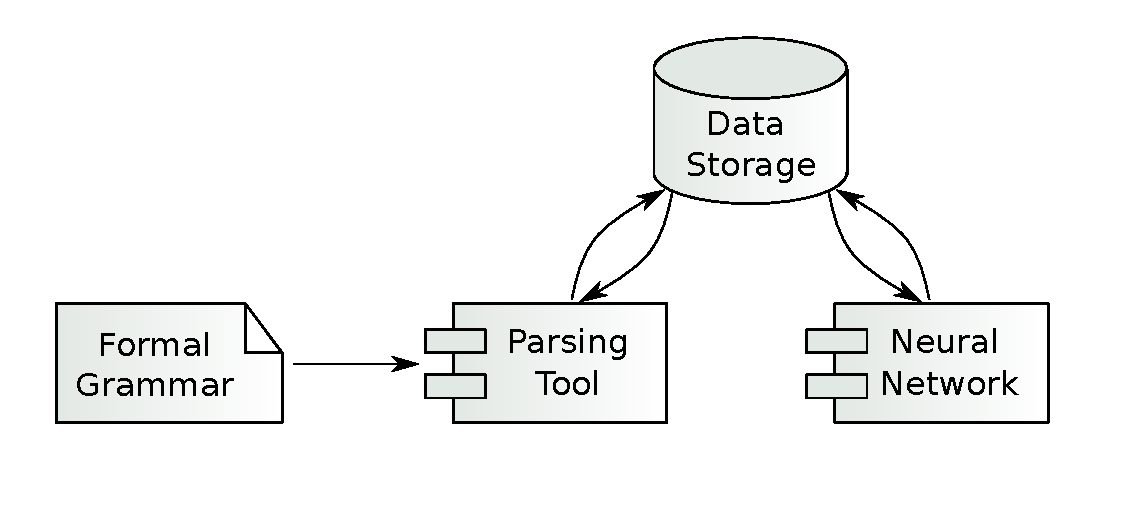
\includegraphics[width=12.0cm]{pics/diagram.pdf}
\caption{Архитектурные компоненты предложенного подхода}
\label{diagram}
\end{center}
\end{figure} 

Одной из потенциальных областей применения такого подхода является биоинформатика, в частности, различные задачи анализа РНК, где в качестве символьных последовательностей можно рассмотреть нуклеотидные цепочки РНК различных организмов, а в качестве синтаксической структуры --- биологическую вторичную структуру молекулы РНК. В текущей работе исследуется возможность применения описанного выше подхода для решения задачи предсказания вторичной структуры РНК. Далее будет описана разработанная для этого архитектура решения, включающая в себя два основных шага: задание грамматики для поиска характерных элементов вторичной структуры, а затем -- проектирование и обучение нейронных сетей, генерирующих для последовательности РНК максимально близкую к реальной вторичную структуру на основе полученных с помощью парсера данных.

\subsection{Формальная грамматика}
Первичная структура молекулы РНК представляет собой цепочку из нуклеотидов четырех типов (аденин, цитозин, гуанин и урацил), что в терминах синтаксического анализа есть последовательность символов алфавита \{A, C, G, U\}; вторичная же структура образовывается вследствие того, что некоторые участки первичной соединяются между собой, формируя рекурсивную композицию из шпилек разного размера и степени вложенности. Обобщенный вид таких шпилек может быть формализован средствами достаточно простой контекстно-свободной грамматики, каковой является используемая в данной работе грамматика $G_0$ (рис.~\ref{gram}). Грамматика учитывает только Уотсон-Криковские правила формирования нуклеотидных пар $A-U$, $C-G$ (строка \textbf{5}) и описывает рекурсивные композиции шпилек высоты от трех и более (строки \textbf{7-12}). Размер петли внутри шпильки лежит в пределах от одного до двадцати нуклеотидов, и такую же длину имеют последовательности, расположенные между любыми двумя шпильками (строка \textbf{2}). Эти числа были выбраны путем балансирования между следующими двумя соображениями: соответствие эмпирическим наблюдениям биологических данных и адекватность напрямую зависящих от длины и сложности грамматики временных затрат на работу парсера. По тем же причинам в $G_0$ не были включены неканонические нуклеотидные связи, которые могут встречаться в реальной вторичной структуре РНК --- для того, чтобы учесть все возможные пары нуклеотидов, придется ввести большое количество правил, имеющих вероятностную природу. Кроме того, средствами контекстно-свободных грамматик невыразимы псевдоузлы, однако псевдоузел есть комбинация из двух шпилек, следовательно, $G_0$, не описывая псевдоузел как единое целое, позволяет, тем не менее, выделить из входной последовательности обе составляющие его подстроки. Здесь становится понятным основное отличие нашего подхода от классического использования формальных грамматик в данной области~\cite{knudsen1999rna,dowell2004evaluation,rivas2000language} --- мы не пытаемся ни смоделировать вторичную структуру целиком, ни описать все возможные закономерности ее образования, но разбиваем ее на простые составные части, синтезировать из которых более сложные объекты предлагается уже с помощью нейронных сетей, что кратно уменьшает интеллектуальные и вычислительные затраты на синтаксический анализ.

\begin{figure}[h]
\begin{Verbatim}[numbers=left,xleftmargin=5mm]
s1: stem<s0>
any_str : any_smb*[1..20]
s0: any_str | any_str stem<s0> s0
any_smb: A | U | C | G
stem1<s>: A s U | G s C | U s A | C s G 
stem2<s>: stem1< stem1<s> >
stem<s>:  
      A stem<s> U 
    | U stem<s> A 
    | C stem<s> G 
    | G stem<s> C 
    | stem1< stem2<s> >  
\end{Verbatim}
\caption{Контекстно-свободная грамматика $G_0$ для описания шпилек вторичной структуры РНК}
\label{gram}
\end{figure}

Рассмотрим теперь формальный вид и практический смысл результата работы синтаксического анализатора для вышеописанной грамматики и последовательности РНК некоторого организма. Синтаксический анализ в данном случае используется для поиска всех подстрок входной строки, выводимых из стартового нетерминала $s1$ грамматики $G_0$, иными словами, для поиска тех участков этой строки, которые, в терминах $G_0$, могут свернуться в шпильки при формировании вторичной структуры. Формально, для входной строки $w$ парсер заполнит верхнетреугольную булеву матрицу --- матрицу разбора $M_P$, где $M_P[i,j]=1 \iff$ подстрока $w[i..j]$ выводится в $G_0$. Так как интересующие нас шпильки должны иметь высоту от трех, каждой шпильке высоты $n$ в матрице разбора будет соответствовать цепочка из $n - 2$ единиц. На рис.~\ref{mtrx} представлен результат работы парсера для изображенного на рис.~\ref{rna_a} случая последовательности, сворачивающейся в шпильку высоты четыре. Каждой нуклеотидной связи, образующей шпильку высоты от трех (сплошные линии голубого цвета), соответствует единица в ячейке матрицы разбора, при этом очевидно, что шпилька высоты три инкапсулирует в себе шпильки высоты два и один, обозначенные на рисунке пунктирными линиями. Помимо уже знакомой нам шпильки с рис.~\ref{rna_a}, в данной строке парсер обнаружил еще одну выводимую в грамматике подстроку (единица в позиции $[0,11]$): таким образом, для рассматриваемой цепочки существует два теоретически возможных варианта свертки, из которых реализованным на практике оказался только один.

\begin{figure}[h]
\begin{center}
\centering
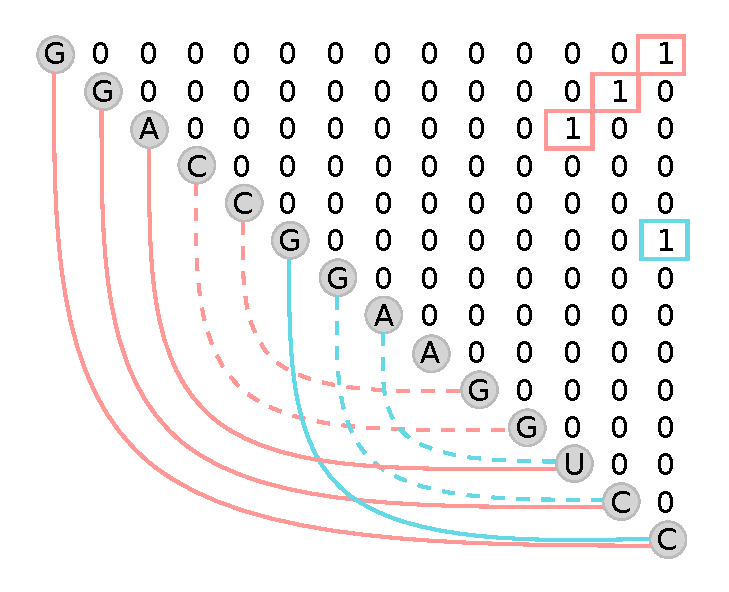
\includegraphics[width=10.0cm]{pics/matrix.pdf}
\caption{Матрица разбора для последовательности РНК}
\label{mtrx}
\end{center}
\end{figure} 
\vspace{3mm}

Остановимся в контексте предложенного подхода на проблеме обработки псевдоузлов, которые, как уже упоминалось ранее, не выводимы в используемой грамматике $G_0$. На рис.~\ref{pk_a} представлен пример последовательности, сворачивающейся в псевдоузел, а на рис.~\ref{pk_b} --- соответствующая данной последовательности матрица разбора. Рассматриваемый псевдоузел состоит из двух взаимопересекающихся шпилек высоты три и четыре, каждая из которых по отдельности выводима в $G_0$ и, следовательно, будет отражена в матрице разбора одной и двумя единицами соответственно. Несмотря на то, что на этапе синтаксического анализа еще не известно, образуют ли эти две найденные шпильки псевдоузел или же являются просто двумя теоретически возможными вариантами свертки цепочки, для нашего подхода предсказание псевдоузлов не становится ни сложностью, ни ограничением, так как матрицы разбора содержат всю необходимую о них информацию, которая должна быть более четко интерпретирована уже на этапе анализа данных нейронными сетями.

\captionsetup[subfigure]{justification=centering}
\begin{figure}[h]
\centering
\begin{subfigure}{.3\textwidth}
  \centering
  \fbox{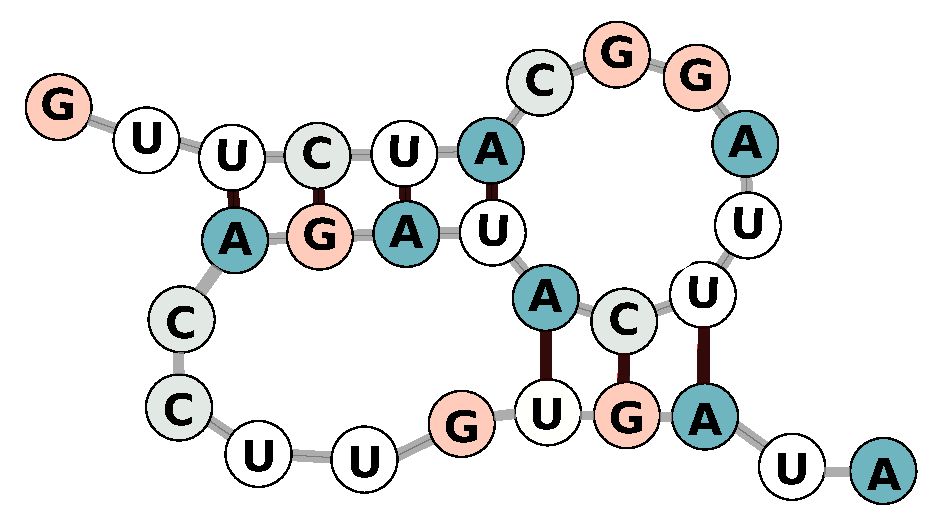
\includegraphics[width=.9\linewidth]{pics/pk.pdf}}
  \caption{Псевдоузел}
  \label{pk_a}
\end{subfigure}%
\begin{subfigure}{.7\textwidth}
  \centering
  \fbox{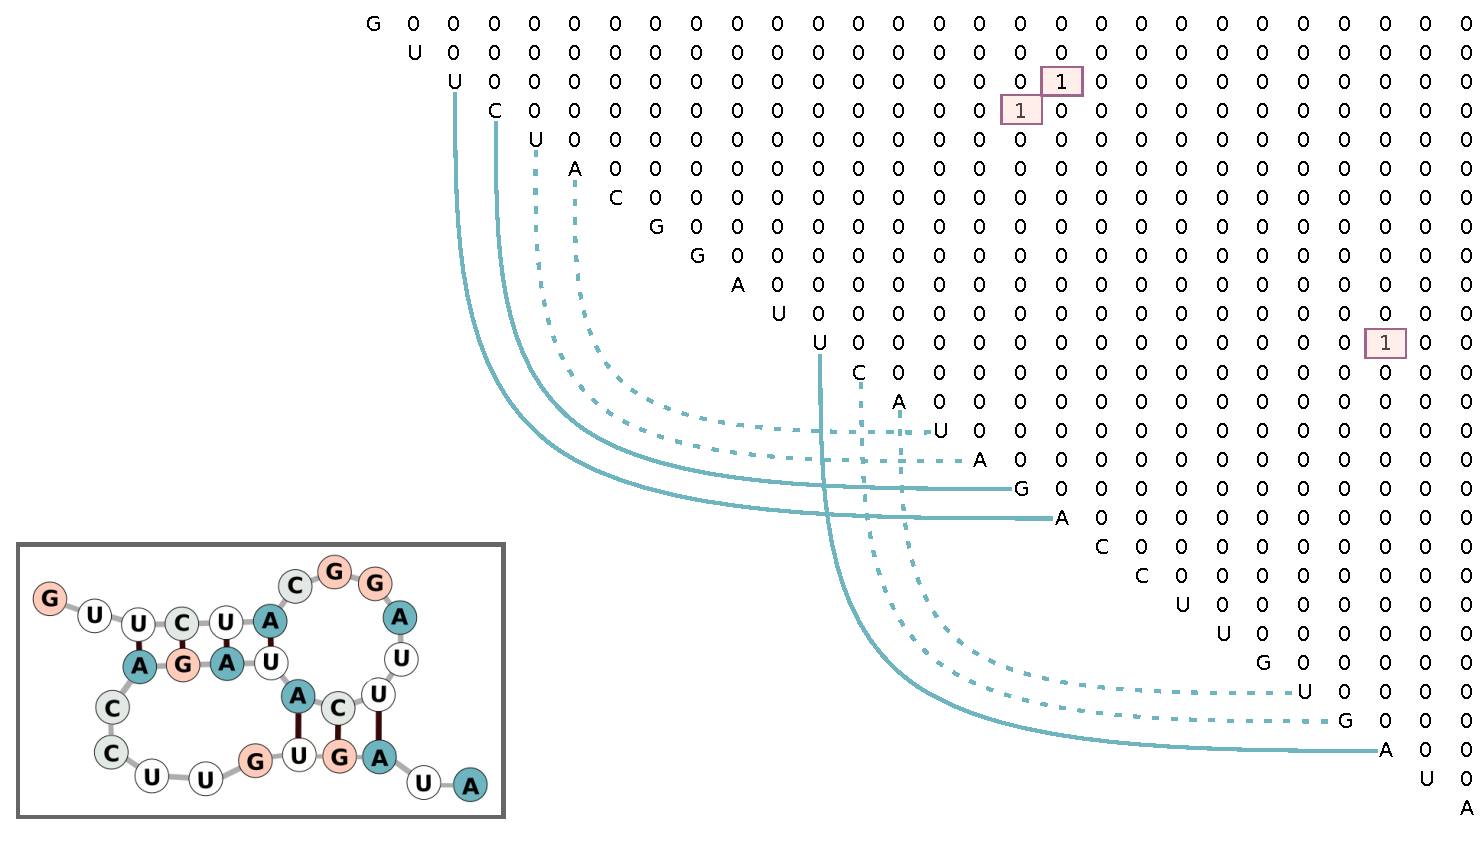
\includegraphics[width=.9\linewidth]{pics/matrix2.pdf}}
  \caption{Матрица разбора для последовательности с псевдоузлом}
  \label{pk_b}
\end{subfigure}
\caption{Обработка псевдоузлов в рамках предложенного подхода}
\label{pk}
\end{figure}

Таким образом, матрицы разбора хранят информацию о всех возможных расположениях шпилек вторичной структуры во входных последовательностях, однако на данный момент это только теоретические, искусственные объекты, для соотнесения которых с реальными биологическими данными требуется последующая обработка, и об этом будет подробно рассказано в следующем разделе.

\subsection{Нейронная сеть}
На данном этапе поставленная задача конкретизируется до следующей --- разработать нейронную сеть, которая принимает на вход матрицы, полученные синтаксическим анализатором по грамматике $G_0$ для некоторого набора последовательностей РНК, и, обучаясь на вторичных структурах, предоставленных в качестве эталонных для рассматриваемых последовательностей, оптимизирует параметры для преобразования матриц разбора в корректные вторичные структуры. Данный раздел посвящен описанию всех тонкостей этого процесса. 

\subsubsection{Подготовка данных} 
Входные данные для нейросети (матрицы разбора) были описаны в прошлом разделе, и теперь необходимо определить источник и формат эталонных данных. Существуют специализированные биологические базы данных, в которых размещены цепочки РНК различных организмов вместе с их извлеченными из природного материала или же полученными надежными методами вторичными структурами. Такие данные оптимальны для валидации, а, следовательно, и для обучения предсказывающих вторичную структуру алгоритмов. 

Как правило, в базах данных вторичные структуры РНК хранятся в скобочной (dot-bracket) нотации, из которой легко получить еще один классический формат  представления вторичной структуры --- так называемую матрицу контактов (contact map). Матрица контактов описывает наличие или отсутствие связи между каждыми двумя нуклеотидами последовательности: формально, для строки $w$ это верхнетреугольная булева матрица $M_C$, где $M_C[i,j]=1 \iff w[i]$ и $w[j]$ образуют пару во вторичной структуре. Как было описано в прошлом разделе, результат работы парсера на входной строке $w$ --- верхнетреугольная булева матрица $M_P$, где $M_P[i,j]=1 \iff w[i..j]$ свернется в шпильку по правилам грамматики. Нетрудно проверить, что наличие контакта между нуклеотидами $w[i]$ и $w[j]$ эквивалентно тому факту, что последовательность $w[i..j]$ является шпилькой, поэтому, несмотря на то, что наше определение вторичной структуры как композиции вложенных шпилек не относится к общеупотребимым, матрицу разбора можно также описать как матрицу контактов, формируемых только выразимыми в грамматике элементами. Таким образом, использование матричного представления вторичной структуры при подготовке эталонных данных для нейронной сети представляется самым удобным в свете специфики используемых в качестве входных данных матриц разбора. 

Для наглядности и удобства применения нейронных сетей мы предлагаем смотреть на матрицу контактов и матрицу разбора как на изображения: пикселями белого цвета обозначим позиции в матрицах с единицами, черного --- с нулями. Матрицы разбора содержат $n - 2$ единицы для каждой шпильки высоты $n>3$, следовательно, в качестве предобработки перед обучением нейросети для каждой единицы в матрице разбора следует добавить еще две единицы в направлении главной диагонали. Кроме того, сама нуклеотидная последовательность РНК может содержать некоторую важную информацию, поэтому предлагается закодировать ее на главной диагонали изображений равноотстающими друг от друга серыми пикселями. 

На рисунке~\ref{struc} продемонстрировано, как для одной и той же последовательности РНК будут выглядеть входной и эталонный образцы для нейронной сети, а также показана визуализация соответствующей вторичной структуры. Контакты, относящиеся к трем присутствующим в рассматриваемой цепочке шпилькам, на всех изображениях выделены голубым, сиреневым и розовым цветами. Данный рисунок является наглядным примером того, что далеко не все найденные парсером шпильки будут представлены в реальной вторичной структуре (белые пиксели изображения~\ref{struc_c}). Кроме того, видно, что в сгенерированной синтаксическим анализатором матрице отсутствует несколько эталонных контактов: в данном случае это произошло из-за того, что они были образованы непредусмотренными грамматикой неканоническими нуклеотидными парами. 

\captionsetup[subfigure]{justification=centering}
\begin{figure}[h]
\centering
\begin{subfigure}{.3\textwidth}
  \centering
  \fbox{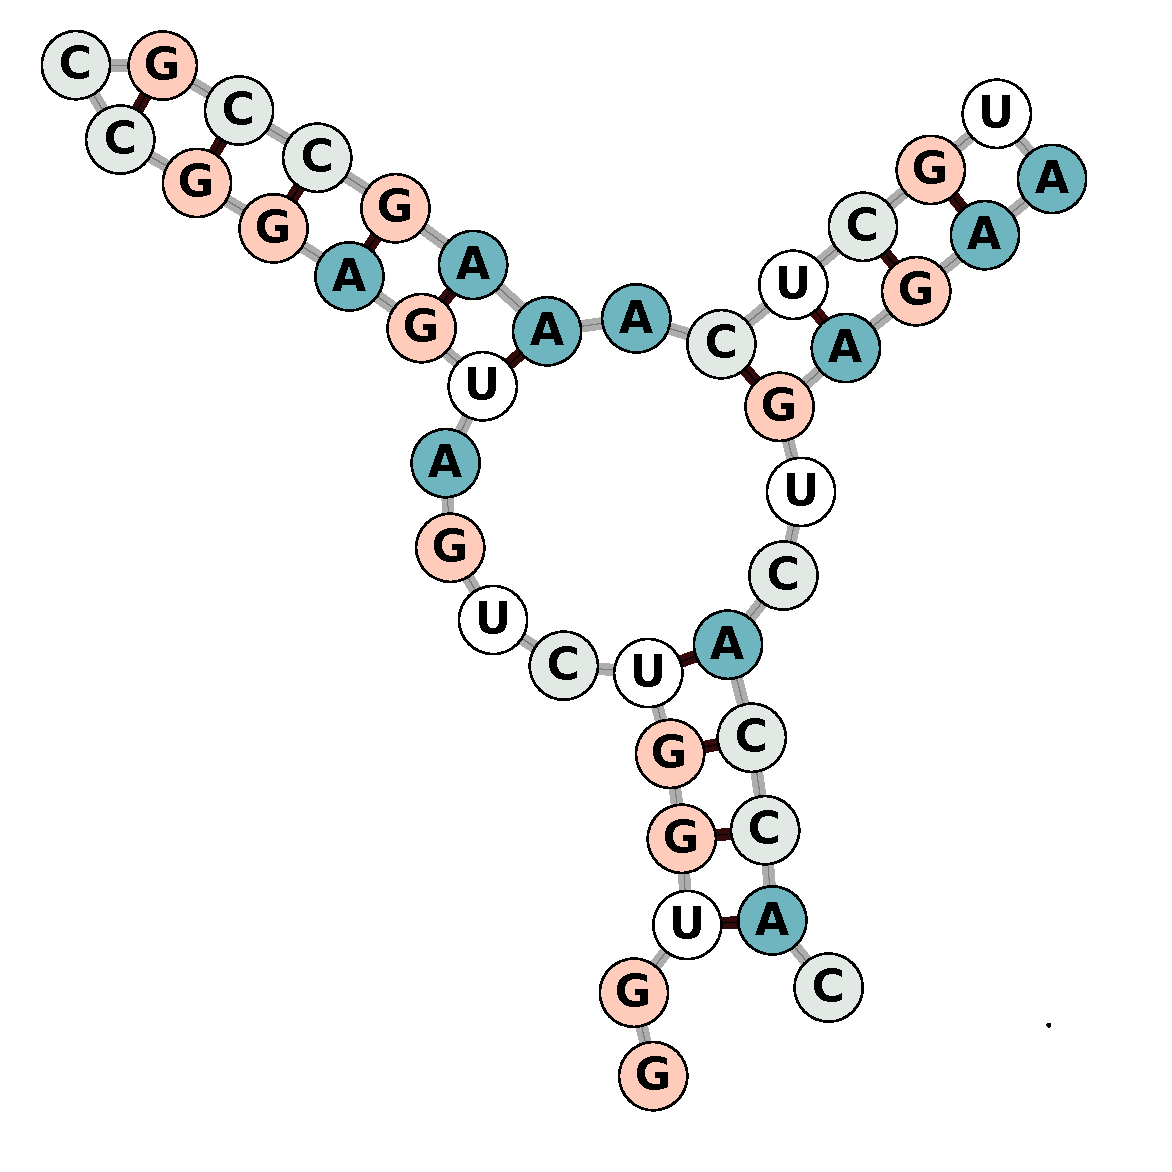
\includegraphics[width=.9\linewidth]{pics/struct.pdf}}
  \caption{Визуализация вторичной структуры}
  \label{struc_a}
\end{subfigure}%
\begin{subfigure}{.3\textwidth}
  \centering
  \fbox{
\includegraphics[width=.9\linewidth]{pics/out.png}}
  \caption{Эталонный  образец \\ для нейросети}
  \label{struc_b}
\end{subfigure}
\begin{subfigure}{.3\textwidth}
  \centering
  \fbox{
\includegraphics[width=.9\linewidth]{pics/in.png}}
  \caption{Входной образец \\ для нейросети}
  \label{struc_c}
\end{subfigure}
\caption{Примеры представления вторичной структуры}
\label{struc}
\end{figure}

Таким образом, в рамках данного исследования перед нейронной сетью стоит задача отфильтровать и дополнить матрицу разбора, сгенерировав корректную матрицу контактов, соответствующую максимально близкой к эталонной вторичной структуре.

\subsubsection{Параллельная остаточная архитектура}
Рассмотрим общую модель нейронной сети, разработанной в рамках данной работы. Входными и выходными данными являются изображения, и для решения поставленной задачи необходимо найти достаточно сложные закономерности между элементами данных, находящимися на большом расстоянии друг от друга, поэтому была использована глубокая сверточная сеть. Для оптимизации процесса обучения и повышения скорости сходимости была применена технология остаточных нейронных сетей. В процессе экспериментальных исследований нами было выявлено, что точность результатов значительно повышает использование $n$ остаточных сетей с одинаковой архитектурой, которые обучаются параллельно на одних и тех же данных, находя в них, по всей видимости, немного разные паттерны, а затем соединяются слоем, подсчитывающим линейную комбинацию их $n$ выходов и передающим ее уже общему остаточному блоку, завершающему обработку данных. Такая новая параллельная архитектура представлена на рис.~\ref{nn}; там же показано, как выглядит типичный остаточный блок (residual unit) нейронной сети, состоящий из пяти сверточных слоев с постепенно убывающими количеством фильтров и размером ядра свертки. В данной работе была использована модель, состоящая из четырех остаточных сетей с пятью одинаковыми блоками в каждой.

\begin{figure}[h]
\begin{center}
\centering
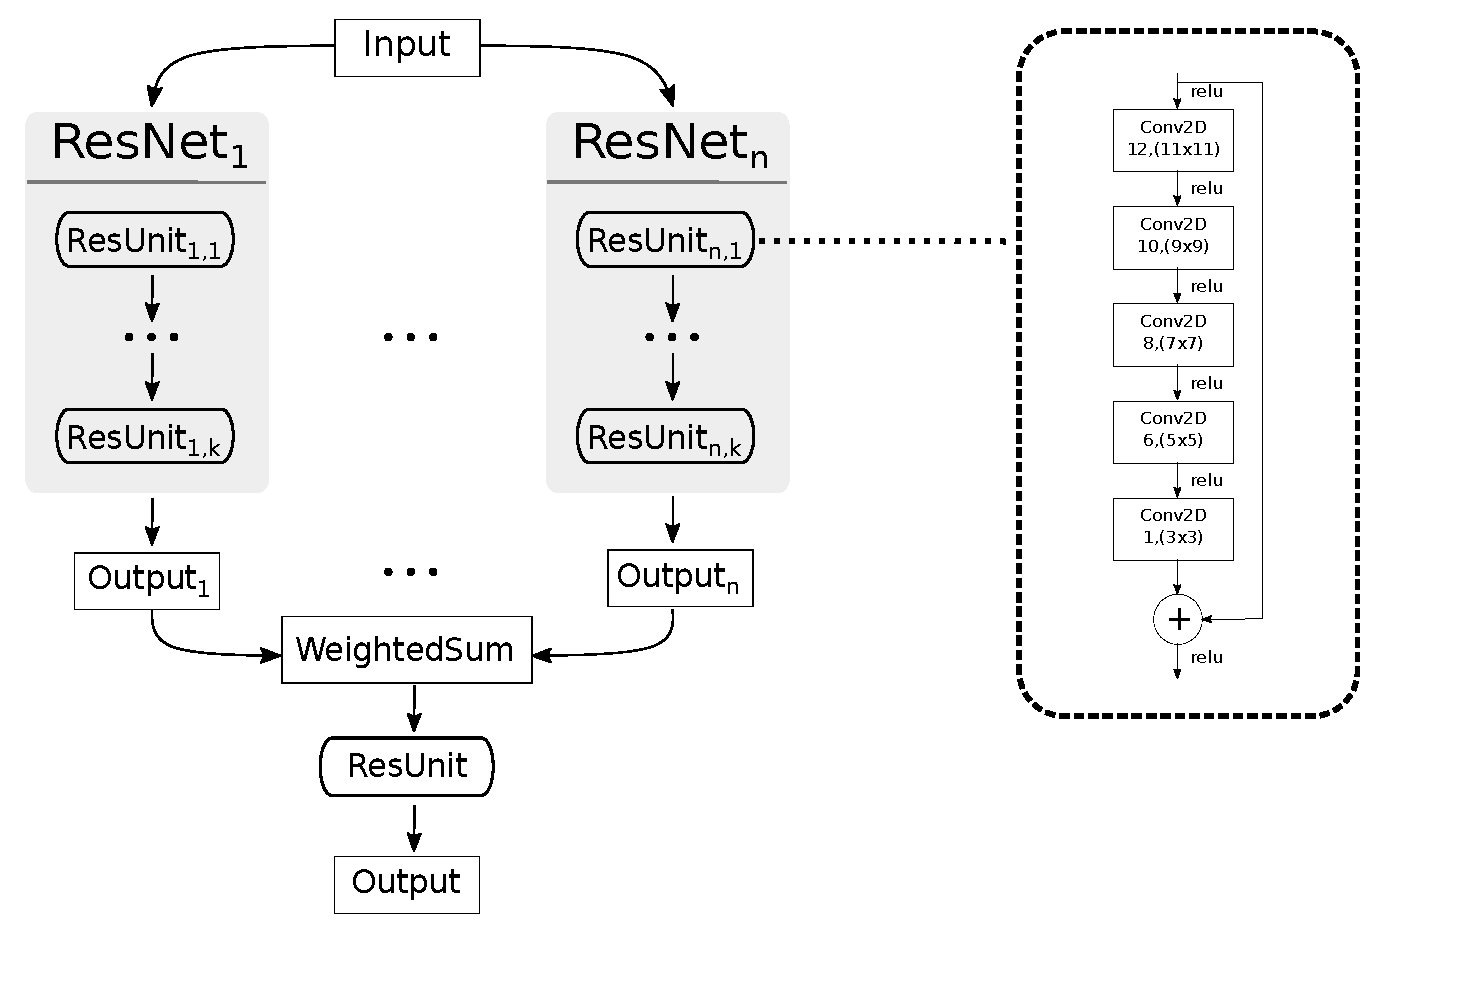
\includegraphics[width=15cm]{pics/nn.pdf}
\caption{Параллельная остаточная нейронная сеть}
\label{nn}
\end{center}
\end{figure} 
\section{Implementation Details}

Details on implementation. 

Architecture.
\section{Алгоритм поиска путей с КС ограничениями}
\label{section:algo_impl}

В данной секции предлагается рассмотреть основные детали реализации алгоритма~\cite{inbook:kronecker_cfpq_adbis} поиска путей с КС ограничениями через тензорное произведение на GPU с использованием библиотеки cuBool, особенности реализации которой были представлены в предыдущей главе..

Реализация алгоритма написана на языке Python с использованием пакета \textbf{pycubool}.
Программа, исполняемая Python-интерпретатором, задает только последовательность вызовов операций.
Вычислительно-интенсивные части алгоритма выполняются на GPU в рамках библиотеки, 
поэтому решение в целом остается производительным.
 
На вход алгоритм получает граф и КС грамматику. 
Граф представлен в виде булевой матричной декомпозиции матрицы смежности графа.
КС грамматика закодирована в виде рекурсивного автомата. 
Его матрица переходов также представлена в булевой матричной декомпозиции.
На выходе алгоритм возвращает матрицу смежности графа достижимости, а также индекс, 
который позволяет восстанавливать все пути в графе в соответствии с входной грамматикой.

Также с использованием \textbf{pycubool} реализован классический матричный алгоритм Рустама Азимова~\cite{inproceedings:matrix_cfpq}, требуемый для корректного сравнения производительности с алгоритмом на основе тензорного произведения.

Реализации упомянутых алгоритмов доступны в рамках открытого проекта \textbf{CFPQ-PyAlgo}~\cite{net:cfpq_py_algo}.
Данный проект предоставляет инфраструктуру для осуществления замеров производительности, а также для загрузки и конвертации данных, требуемых для экспериментов.
Архитектура данного стенда представлена на рис.~\ref{fig:cfpq_py_algo}. 
Тестовый стенд позволяет использовать различные библиотеки и инструменты для реализации в модуле  \textbf{Algorithms} алгоритмов поиска путей с КС ограничениями. Также стенд предоставляет утилиты для загрузки входных графов в модуле \textbf{Grpah}, для загрузки грамматик и преобразования их в требуемый формат в модуле \textbf{Grammar} соответственно.
Пакет \textbf{CFPQ-Data}~\cite{net:cfpq_data} используется для загрузки из локального или удаленного хранилища актуальной версии набора данных для замеров.

\begin{figure}[]
    \centering
    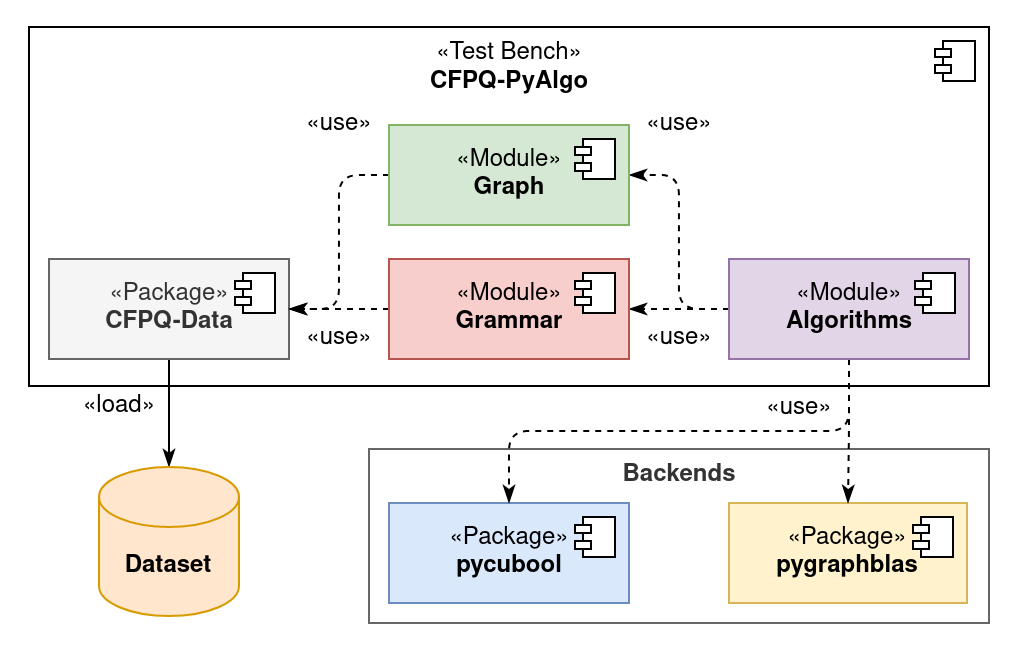
\includegraphics[width=0.9\textwidth]{images/cfpq_pyalgo.png}
    \caption{Архитектура стенда для тестирования алгоритмов}
    \label{fig:cfpq_py_algo}
\end{figure}

В инфраструктуре уже доступны базовые реализации алгоритма Рустама Азимова~\cite{inproceedings:matrix_cfpq} и алгоритма на основе тензорного произведения для вычислений на CPU. 
В качестве основы эти реализации используют пакет \textbf{pygraphblas}, который предоставляет доступ к примитивам разреженной линейной алгебры из стандарта GraphBLAS API~\cite{paper:graphblas_foundations} и его эталонной реализации SuiteSparse~\cite{article:suite_sparse_for_graph_problems}. 
Данные реализации алгоритмов также используются для проведения экспериментального исследования.






\section{Evaluation}

For performance analysis of proposed solution we evaluated some most common graph algorithms using real-world sparse matrix data. 
As a baseline for comparison we chose LAGraph~\cite{szarnyas2021lagraph} in connection with SuiteSparse~\cite{10.1145/3322125} as a CPU tool, Gunrock~\cite{7967137} and GraphBLAST~\cite{yang2019graphblast} as a Nvidia GPU tools. 
Also, we tested algorithms on several devices with distinct OpenCL vendors in order to validate portability of the proposed solution. 
In general, these evaluation intentions are summarized in the following research questions. 

\vspace{0.2cm}
\begin{itemize}
    \item[\textbf{RQ1}] What is the performance of the proposed solution relative to existing tools for both CPU and GPU analysis?
    
    \item[\textbf{RQ2}] What is the portability of the proposed solution with respect to various device vendors and OpenCL runtimes?
\end{itemize}

\subsection{Evaluation Setup}

For evaluation, we use a PC with Ubuntu 20.04 installed, which has 3.40Hz Intel Core i7-6700 4-core CPU, DDR4 64Gb RAM, and Nvidia GeForce GTX 1070 GPU with 8Gb VRAM. 
Host programs were compiled with GCC 9.3.0 compiler. Programs using CUDA were compiled with GCC 8.4.0 and Nvidia NVCC 10.1.243 compiler.
Release mode and maximum optimization level was enabled for all tested programs. 
Data loading time, preparation, format transformations and host-device initial communications are excluded from time measurements. 
All tests are averaged across 10 runs.
Additional warm-up run for each test execution is excluded from measurements.

\subsection{Graph Algorithms}

For preliminary study \textit{breadth-first search} (bfs) and \textit{triangles counting} (tc) algorithms were chosen, since they allows analyse the performance of \textit{vxm} and \textit{mxm} operations, rely heavily on \textit{masking}, and utilize \textit{reduction} or \textit{assignment}. 
BFS implementation utilizes automated vector storage from sparse to dense switch and only \textit{}{push optimization}. 
TC implementation uses masked \textit{mxm} of source lower-triangular matrix with second transposed argument.

\subsection{Dataset}

Nine graph matrices were selected from the Sparse Matrix Collection at University of Florida~\cite{dataset:10.1145/2049662.2049663}. 
Information about graphs is summarized in Table~\ref{dataset:info}. 
All datasets are converted to undirected graphs. 
Self-loops and duplicated edges are removed.

\begin{table}[htbp]
\caption{Dataset description.} 
\begin{center}
    \rowcolors{2}{black!2}{black!10}
    \begin{tabular}{|l|r|r|r|}
    \hline
    Dataset & Vertices  & Edges & Max Degree \\
    \hline
    \hline
    coAuthorsCiteseer & 227.3K &   1.6M &    1372 \\
    coPapersDBLP      & 540.4K &  30.4M &    3299 \\
    hollywood-2009    &   1.1M & 113.8M &  11,467 \\
    roadNet-CA        &   1.9M &   5.5M &      12 \\
    com-Orkut         &     3M &   234M &   33313 \\
    cit-Patents       &   3.7M &  16.5M &     793 \\
    rgg\_n\_2\_22\_s0 &   4.1M &  60.7M &      36 \\
    soc-LiveJournal   &   4.8M &  68.9M &  20,333 \\
    indochina-2004    &   7.5M & 194.1M & 256,425 \\
    \hline
    \end{tabular}
    \label{dataset:info}
\end{center}
\end{table}

\subsection{Results}

Table~\ref{results} presents results of the evaluation and compares performance of Spla against other tool on different execution platforms.
Tools are grouped by the type of the device for the execution, where either Nvidia GPU or Intel CPU are used. 
Cell left empty if tested tool failed to analyse graph due to \textit{out of memory} exception.

In general, Spla BFS shows acceptable performance, especially on graphs with large vertex degree, such as soc-LiveJournal and com-Orkut.
On graphs roadNet-CA and rgg it has a significant performance drop due to the nature of underlying algorithms and data structures. 
Firstly, library utilizes immutable data buffers. Thus, iteratively updated dense vector of reached vertices must be copied for each modification, what dominates the performance of the library on a graph with large search depth. 
Secondly, Spla BFS does not utilise \textit{pull optimization}, what is critical in a graph with relatively small search frontier. 

Spla TC has a good performance on GPU, which is better in all cases that reference SuiteSparse solution. 
But in most tests GPU competitors, especially Gunrock, show smaller processing times. 
GraphBLAST shows better performance as well. 
Library utilises masked SpGEMM algorithm, the same as in GraphBLAST, but without \textit{identity} element to fill gaps. 
Library explicitly stores all non-zero elements, and uses mask to reduce only non-zero while evaluating dot products of rows and columns. 
What causes extra divergence inside work groups. 
On Intel device Spla shows better performance compared to SuiteSparse on com-Orkut, cit-Patents and soc-LiveJournal. 
A possible reason is the large lengths of processed rows and columns in the product of matrices.

Gunrock shows nearly best average performance due to its specialized and optimized algorithms.
Also, it has good time characteristics on a mentioned earlier roadNet-CA and rgg in BFS algortihm. 
GraphBLAST follows Gunrock and show good performance as well. 
But it runs out of memory on a two significantly large graphs con-Orkut and indochina-2004. 
Spla does not rut out of memory on any test due to simplified storage scheme.

\begin{table}[htbp]
\caption{Graph algorithms evaluation results.\\Time in milliseconds (lower is better).} 
\begin{center}
    \begin{tabular}{|l|r|r|r|r|r|}
    \hline
    \multirow{2}{*}{Dataset} & \multicolumn{3}{c|}{Nvidia} & \multicolumn{2}{c|}{Intel} \\
    \cline{2-6}
    & GR & GB & SP & SS & SP \\
    \hline
    \hline
    \multicolumn{6}{|c|}{BFS} \\
    \hline
    \rowcolor{black!10} hollywood-2009    &  20.3 &  82.3 &   36.9 &   23.7 &   303.4 \\
    \rowcolor{black!2 } roadNet-CA        &  33.4 & 130.8 & 1456.4 &  168.2 &   965.6 \\
    \rowcolor{black!10} soc-LiveJournal   &  60.9 &  80.6 &   90.6 &   75.2 &  1206.3 \\
    \rowcolor{black!2 } rgg\_n\_2\_22\_s0 &  98.7 & 414.9 & 4504.3 & 1215.7 & 15630.1 \\
    \rowcolor{black!10} com-Orkut         & 205.2 & -- -- &  117.9 &   43.2 &   903.6 \\
    \rowcolor{black!2 } indochina-2004    &  32.7 & -- -- &  199.6 &  227.1 &  2704.6 \\
    \hline
    \hline
    \multicolumn{6}{|c|}{TC} \\
    \hline
    \rowcolor{black!10} coAuthorsCiteseer &   2.1 &    2.0 &    9.5 &    17.5 &    64.9 \\
    \rowcolor{black!2 } coPapersDBLP      &   5.7 &   94.4 &  201.9 &   543.1 &  1537.8 \\
    \rowcolor{black!10} roadNet-CA        &  34.3 &    5.8 &   16.1 &    47.1 &   357.6 \\
    \rowcolor{black!2 } com-Orkut         & 218.1 & 1583.8 & 2407.4 & 23731.4 & 15049.5 \\
    \rowcolor{black!10} cit-Patents       &  49.7 &   52.9 &   90.6 &   698.3 &   684.1 \\
    \rowcolor{black!2 } soc-LiveJournal   &  69.1 &  449.6 &  673.9 &  4002.6 &  3823.9 \\
    \hline
    \hline
    \multicolumn{6}{l}{Tools: Gunrock (GR), GraphBLAST (GB), SuiteSparse (SS), Spla (SP).} \\
    \end{tabular}
    \label{results}
\end{center}
\end{table}
 
% Two GPU

% \begin{table}[htbp]
%     \caption{Table Type Styles}
%     \begin{center}
%     \begin{tabular}{|c|c|c|c|}
%     \hline
%     \textbf{Table}&\multicolumn{3}{|c|}{\textbf{Table Column Head}} \\
%     \cline{2-4} 
%     \textbf{Head} & \textbf{\textit{Table column subhead}}& \textbf{\textit{Subhead}}& \textbf{\textit{Subhead}} \\
%     \hline
%     copy& More table copy$^{\mathrm{a}}$& &  \\
%     \hline
%     \multicolumn{4}{l}{$^{\mathrm{a}}$Sample of a Table footnote.}
%     \end{tabular}
%     \label{tab2}
%     \end{center}
% \end{table}

\section{Conclusion}

In this paper we present a library for sparse Boolean linear algebra which implements such basic operations as matrix-matrix multiplication and element-wise matrix-matrix addition in both Cuda and OpenCL.
Evaluation shows that our Boolean-specific implementations faster and require less memory than generic, not the Boolean optimized, operations from state-of-the-art libraries. 
Thus, the specialization of operations for this data type makes sense. 

The first direction of the future work is to integrate all parts (OpenCL and Cuda backends) into a single library and improve its documentation and prepare to publish.
Moreover, it is necessary to extend the library with other operations, including matrix-vector operations, masking, and so on.
As a result a Python package should be published.

Another important step is to evaluate the library on different algorithms and devices.
Namely, algorithms for RPQ and CFPQ should be implemented and evaluated on related data sets.
Also, it is necessary to evaluate OpenCL version on FPGA which may require additional technical effort and code changes.

Finally, we plan to discuss with GraphBLAS community possible ways to use our library as a backend for GraphBLAST or SuiteSparse in case of Boolean computations.
Moreover, it may be possible to use implemented algorithms as a foundation for generalization to arbitrary semirings.


% \section{Эксперимент}
% Как мы проверяем, что  всё удачно получилось

% \subsection{Условия эксперимента}
% Железо (если актуально); входные данные, на которых проверяем наш подход; почему мы выбрали именно эти тесты

% \subsection{Исследовательские вопросы (Research questions)}
% Надо сформулировать то, чего мы хотели бы добиться работой (2 штуки будет хорошо):

% \begin{itemize}
% \item Хотим алгоритм, который лучше вот таких-то остальных
% \item Если в подходе можно включать/выключать составляющие, то насколько существенно каждая составляющая влияет на улучшения
% \item Если у нас строится приближение каких-то штук, то на сколько точными будут эти приближения
% \item и т.п.
% \end{itemize}

% \subsection{Метрики}

% Как мы сравниваем, что результаты двух подходов лучше или хуже
% \begin{itemize}
% \item Производительность
% \item Строчки кода
% \item Как часто алгоритм "угадывает" правильную классификацию входа
% \end{itemize}

% Иногда метрики вырожденные (да/нет), это не очень хорошо, но если в области исследований так принято, то ладно.

% \subsection{Результаты}
% Результаты понятно что такое. Тут всякие таблицы и графики

% В этом разделе надо также коснуться Research Questions.

% \subsubsection{RQ1} Пояснения
% \subsubsection{RQ2} Пояснения

% \subsection{Обсуждение результатов}

% Чуть более неформальное обсуждение, то, что сделано. Например, почему метод работает лучше остальных? Или, что делать со случаями, когда метод классифицирует вход некорректно.

% \section{Применение того, что сделано на практике (опциональный)}

% Если применение в лоб не работает, потому что всё изложено чуть более сжато и теоретично, надо рассказать тонкости и правильный метод применения результатов. 

% \section{Угрозы нарушения корректности (опциональный)}

% Если основная заслуга метода, это то, что он дает лучшие цифры, то стоит сказать, где мы могли облажаться, когда проводили численные замеры. 

% \section{Заключение}

% Кратко, что было сделано. Также здесь стоит писать задачи на будущее.

% \textbf{Для курсовых/дипломов.} Также стоит сделать список результатов, который будет 1 к одному соответствовать задачам из раздела~\ref{sec:task}.

% \begin{itemize}
% \item Результат к задаче 1 
% \item Результат к задаче 2
% \item и т.д.
% \end{itemize}

% \nocite{*}
\setmonofont[Mapping=tex-text]{CMU Typewriter Text}
\bibliographystyle{ugost2008ls}
\bibliography{kronecker_cfpq_gpu_diploma}

\end{document}